	
	\subsection*{Question 1}
	
	Recopier et compléter l'arbre de probabilités suivant :
	
\begin{center}
	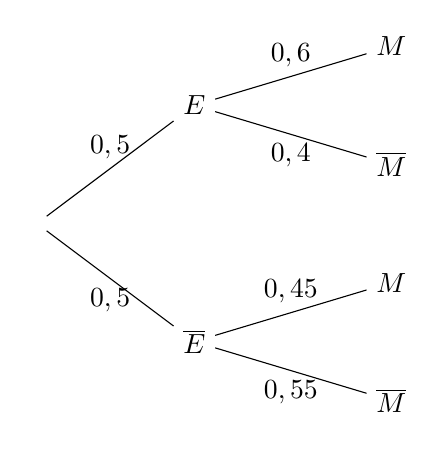
\begin{tikzpicture}
		[level 1/.style={level distance=2cm,
			sibling distance=3cm},
		level 2/.style={level distance=2.5cm,
			sibling distance=1.5cm}]
		\node {} [grow'=right]
		child {node {$E$}
			child {node {$M$}
				edge from parent node[above] {$0,6$}
			}
			child {node {$\overline M$}
				edge from parent node[below] {$0,4$}
			}
			edge from parent node[above] {$0,5$}
		}
		child {node {$\overline E$}
			child {node {$M$}
				edge from parent node[above] {$0,45$}
			}
			child {node {$\overline M$}
				edge from parent node[below] {$0,55$}
			}
			edge from parent node[below] {$0,5$}
		}
		;
	\end{tikzpicture}
\end{center}
	
	\subsection*{Question 2}
	
	On a :
	\begin{align*}
		p(E \cap M) &= p(E) \times p_E(M) \\
		&= 0,5 \times 0,6 = 0,3.
	\end{align*}
	
	\subsection*{Question 3}
	
	On a aussi :
	\begin{align*}
		p(\overline{E} \cap M) &= p(\overline{E}) \times p_{\overline{E}}(M) \\
		&= 0,5 \times 0,45 = 0,225.
	\end{align*}
	
	D'après la loi des probabilités totales :
	\begin{align*}
		p(M) &= p(E \cap M) + p(\overline{E} \cap M) \\
		&= 0,3 + 0,225 = 0,525.
	\end{align*}
	
	\subsection*{Question 4}
	
	On cherche $p_M(E)$ :
	\begin{align*}
		p_M(E) &= \frac{p(M \cap E)}{p(M)} \\
		&= \frac{0,225}{0,525} \approx 0,429.
	\end{align*}
	Soit $p_M(E) \approx 0,43$ au centième près.
	
	\subsection*{Question 5}
	
	On a :
	\begin{align*}
		p(E \cap \overline{M}) &= p(E) \times p_E(\overline{M}) \\
		&= 0,5 \times 0,55 = 0,275.
	\end{align*}
	
	La probabilité de gagner une seule partie est donc :
	\begin{align*}
		1 - (0,3 + 0,275) &= 1 - 0,575 = 0,425.
	\end{align*}
	
	L'espérance mathématique de la variable aléatoire associée est :
	\begin{align*}
		E(X) &= 4 \times 0,3 + 2 \times 0,425 + 0 \times 0,275 \\
		&= 1,2 + 0,85 = 2,05.
	\end{align*}
	
